\documentclass{beamer}

\usetheme{Boadilla}

\newcommand{\bi}{\begin{itemize}}
\newcommand{\ei}{\end{itemize}}
\newcommand{\be}{\begin{enumerate}}
\newcommand{\ee}{\end{enumerate}}
\newcommand{\I}{\item}
\newcommand{\f}{\frame}
\newcommand{\ft}{\frametitle}

\title{Overview of Requirements}
\subtitle{for the FDC Mini-Review}
\author[M.\ Ito]{Mark M.\ Ito}
\date{February 1, 2008}
\institute[JLab]{Jefferson Lab}

\begin{document}

\f{\titlepage}

\f{
  \ft{Outline}
  \bi
  \I physics goals
  \I GlueX detector
  \I reviews: past, present and future
  \I design considerations
  \I specifications
  \I resolution estimates
  \I conclusions
  \ei
}

\f{
  \centerline{\Large physics goals}
}
\f{
  \ft{goals and requirements}

The search for exotic mesons is at a turning
point...experiments...which have reported evidence for exotic mesons
have terminated data taking...new experiments are ahead of
us...[including] the Hall-D experiment at the upgraded JLab
facility...in the medium-range future. --- Eberhard Klempt

  \bi
  \I Map the spectrum of hybrid mesons (gluonic excitations)
    \bi
    \I Start with those with exotic quantum numbers
    \I Make contact with spectroscopy of non-exotic states
    \ei

  \I Analysis will require
    \bi
    \I partial-wave analysis
    \I identification of exclusive final states
    \I detailed understanding of backgrounds
    \I large event samples
    \I confirmation of states in multiple decay channels
    \ei
  \ei
}
\f{
  \ft{lattice mass predictions}
  Lowest mass expected to be $\pi_1(1^{−+})$ at $1.9 \pm 0.2$~GeV
$$
  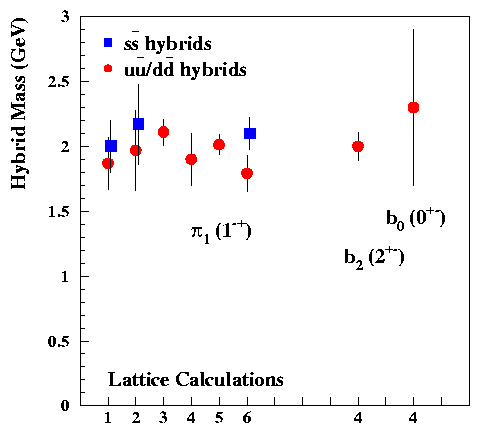
\includegraphics[height=3in]{hybrids_lattice.png}
$$
}
\f{
  \ft{representative kinematics}
$$
  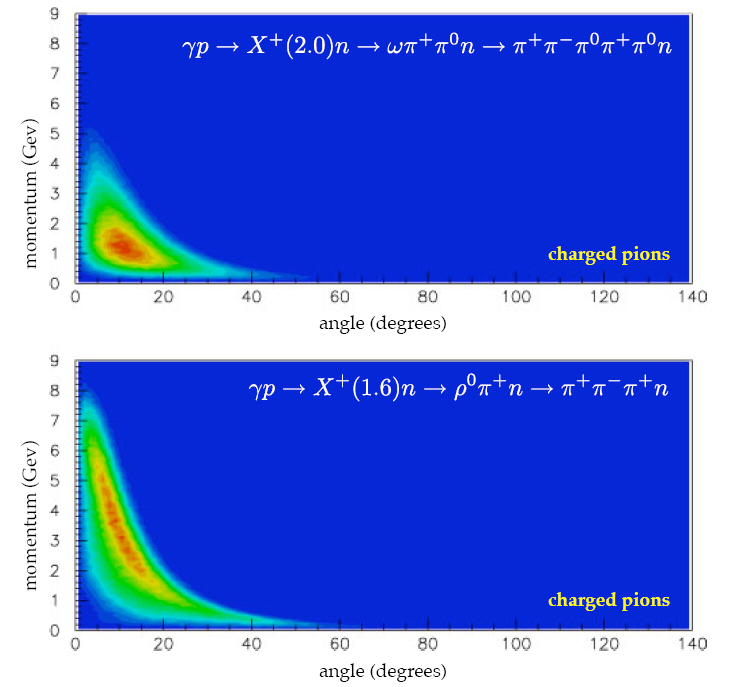
\includegraphics[height=3in]{kinematics.png}
$$
}
\f{
  \ft{anything else?}
  \bi
  \I Hall D a unique facility
    \bi
    \I high-energy tagged photon beam
    \I coherent bremsstrahlung $\Rightarrow$ nearly mono-energetic beam
    \I linear polarization
    \ei
  \I driven to a general purpose detector
    \bi
    \I charged and neutral particle detection
    \I very large acceptance
    \ei
  \I other physics possible!
    \bi
    \I come to the workshop, PHP2008, March 6-8, at JLab
    \I ``Photon-hadron physics with the GlueX detector at Jefferson Lab''
    \ei
  \ei
}
\f{
  \centerline{\Large GlueX detector}
}
\f{
  \ft{the detector}
  $$
  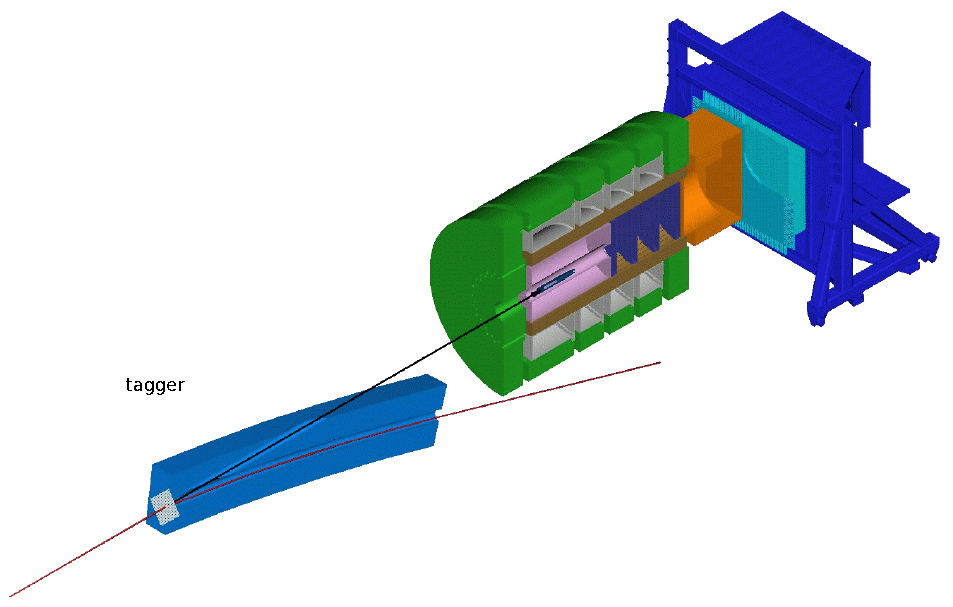
\includegraphics[height=3in]{gluex_detector_3d.png}
  $$
}
\f{
  \ft{elevation view}
  $$
  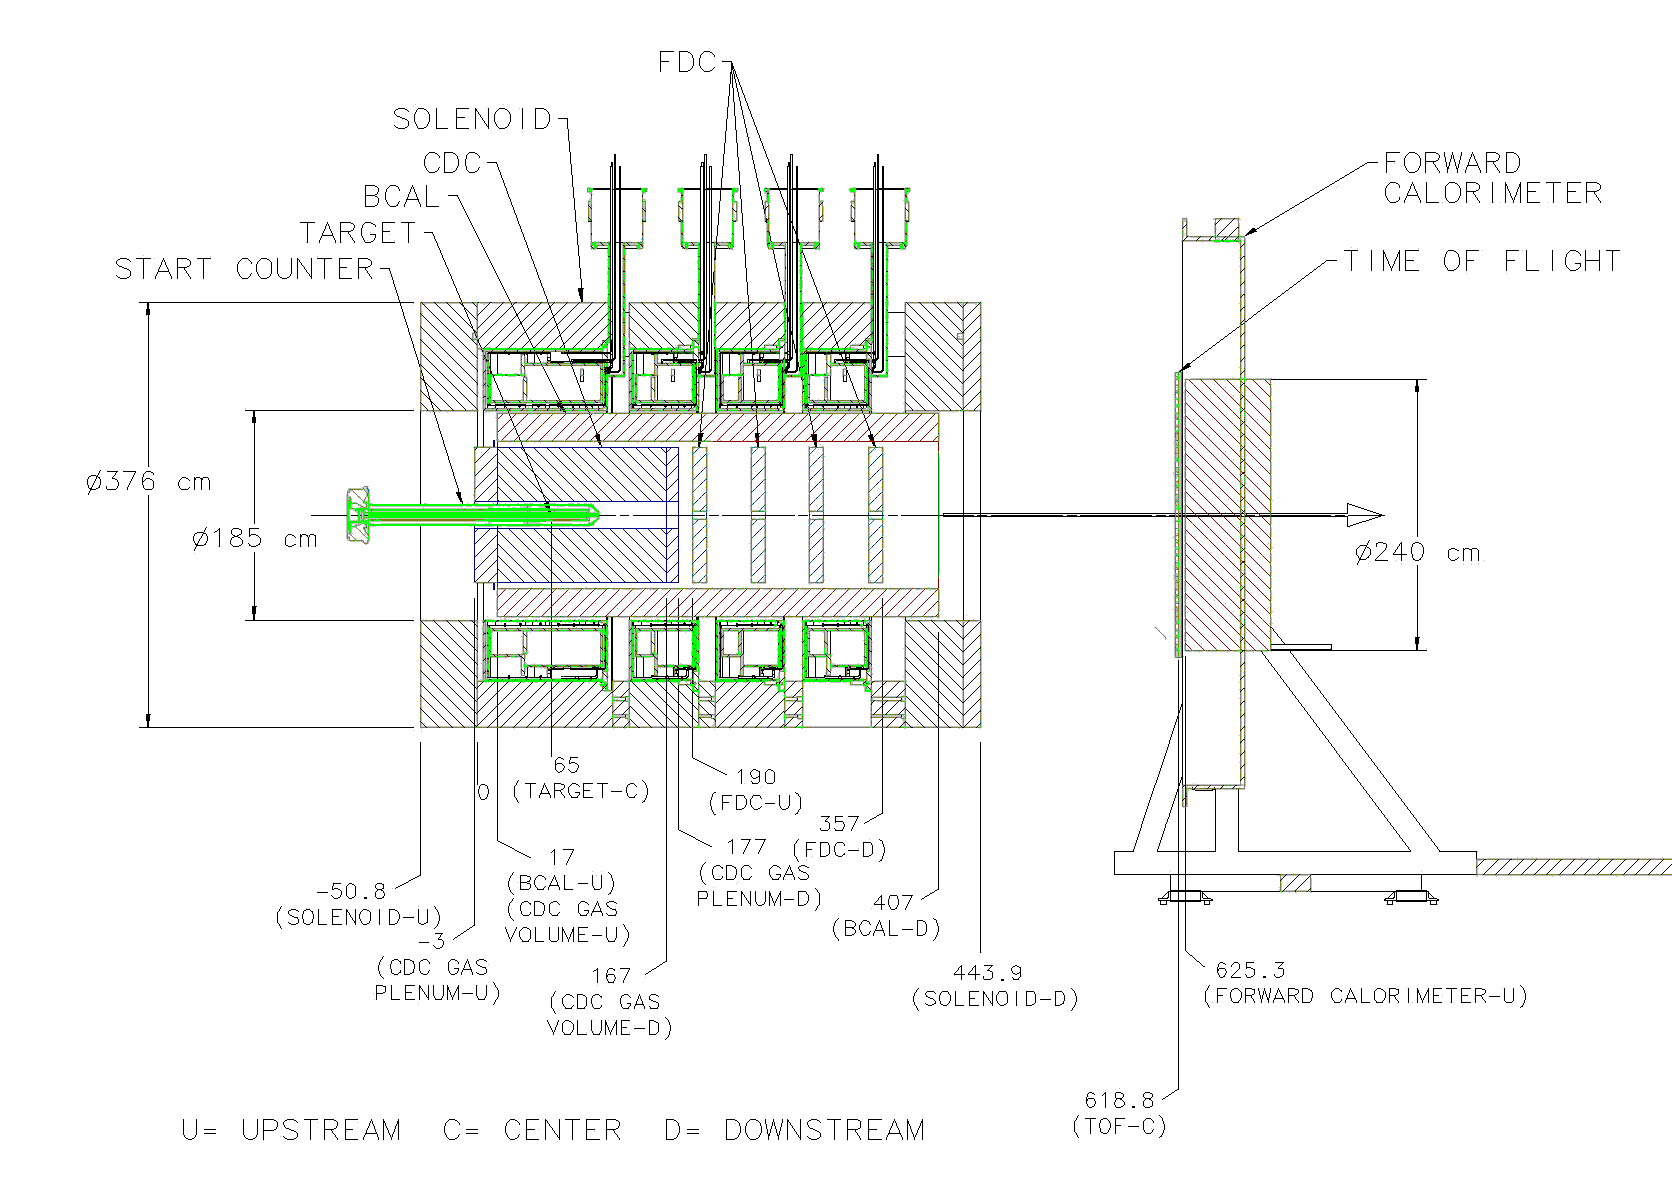
\includegraphics[height=3in]{gluex_detector.png}
  $$
}
\f{
  \centerline{\Large reviews: past, present and future}
}
\f{
  \ft{review roster}
  \bi
  \I \textcolor{red}{Drift Chamber Review, Hall B and D, March 2007}
  \I CD-2 12 GeV Project Review, June 2007
  \I
  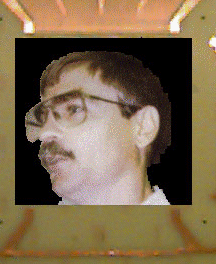
\includegraphics[height=0.5in]{howard_pwc.png}\textcolor{red}{$\leftarrow$FDC
    Mini-Review, February
    2008$\rightarrow$}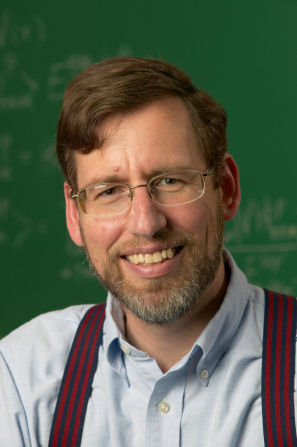
\includegraphics[height=0.5in]{Larry_Weinstein.jpg}
  \I \textcolor{red}{Drift Chamber Review, March 2008}
  \I CD-3 Project Review, June 2008
  \ei
}
\f{
  \ft{Drift Chamber Review, Hall B and D, March 2007}

  Recommendations (Hall D)

  \begin{enumerate}

    \I Priority should be given to studying design modifications that
    would significantly reduce the amount of material in the GlueX
    tracking chambers.

    \I Additional resources and expertise should be applied to the
    development of track reconstruction software for GlueX, and to a
    complete and realistic hit-level simulation of the GlueX
    spectrometer.

  \end{enumerate}
}
\f{
  \centerline{\Large design considerations}
}
\f{
  \ft{really general stuff}
  \bi
  \I characteristics of the acceptance
    \bi
    \I must be large
    \I must be smooth
    \I must be well understood
    \I driven by need to do a partial-wave analysis
    \ei
  \I resolution counts
    \bi
    \I needed for missing mass identification
    \I reduces combinatoric background under narrow resonances
    \I sharpens results from the partial-wave analysis
    \I surprises, unintended benefits, etc.
    \ei
  \I robust pattern recognition
    \bi
    \I robustness $\Leftrightarrow$ simplicity $\Leftrightarrow$
    speed of reconstruction
    \I implications for
      \bi
      \I online level 3 trigger
      \I offline processing speed
      \ei
    \ei
  \ei
}
\f{
  \ft{$\forall$ FDC's}
  \bi
  \I drift chambers
  \I 4 packages
  \I no structural segmentation in azimuth (no $phi$ sectors)
  \I pipeline readout
  \I variations on design work already done for the reference design  
  \I aside: preserve $dE/dx$ for particle ID as an option if possible
  \ei
}
\f{
  \ft{design options}
  \be
  \I two cathode strip planes per wire plane (reference)
    \bi
    \I six anode wire planes per package
    \I twelve cathode strip planes
    \I cathodes at $\pm 75^\circ$
    \I each anode plane rotated $60^\circ$ from previous anode plane
    \I TDC readout for anodes
    \I FADC readout for cathodes
    \ei
  \I no cathode strips (wires only)
    \bi
    \I twelve(?) anode wire planes per package
    \I orientation options
      \be
      \I each plane rotated $60^\circ$ from previous
      \I pairs of planes with half-cell offset, pairs rotated
      $60^\circ$ from previous
      \ee
    \ei
  \I one cathode strip plane per anode wire plane (hybrid)
  \ee
}
\f{
  \ft{pro's and con's}
  \bi
  \I reference design
    \be
    \I position resolution of cathodes in a layer good enough to select single wire in anode plane
    \I cathodes strips and anode wires see the same avalanche
      \bi
      \I can use timing to correlate strips with wires
      \I FADC's on cathode strips give a time measurement
      \I time resolution should be sufficient
      \I especially useful in eliminating isolated single-cell hits
      \ei
    \I momentum resolution is multiple-scattering dominated
    \ee
  \I wires-only design
    \be
    \I cathode strip planes replaced with thin cathode sheets
    \I much less material
    \I tried and true
    \I cost savings due to fewer electronics channels
    \ee
  \ei
}
\f{
  \centerline{\Large specifications}
}
\f{
  \ft{nominal specs}
  \begin{center}
    \begin{tabular}{ll}
      polar angle coverage         &  $1^\circ < \theta < 140^\circ$ \\
      azimuthal angle coverage         & $2\pi$ \\
      momentum resolution &  $\sigma_p/p = 1-3\%$ \\
      position resolution &  $\sigma\approx 150-200 \mu m$
    \end{tabular}
  \end{center}
}
\f{
  \centerline{\Large resolution estimates}
}
\f{
  \ft{placeholder plot: $\sigma_p/p$ vs.\ p (GeV/$c$)}
  $$
  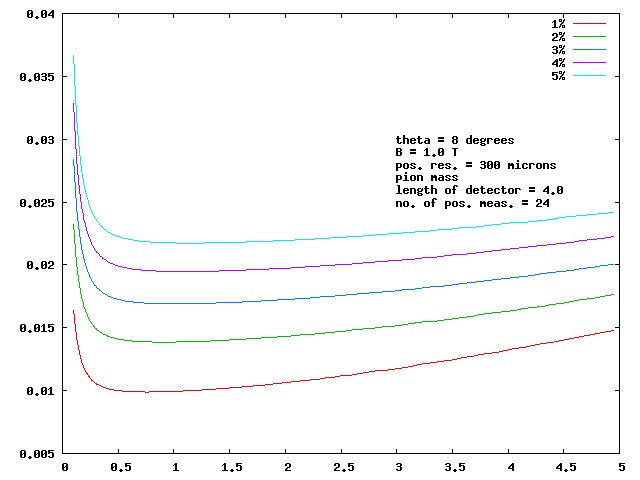
\includegraphics[height=3in]{rezest_1t_4m.jpg}
  $$
}
\f{
  \centerline{\Large conclusions}
}
\f{
  \ft{let me end with...}
  hmmmmm......
}

\end{document}

%%% end of latex file %%%%
